\section{Outils de build : au delà des
Makefile}\label{outils-de-build-au-deluxe0-des-makefile}

\begin{frame}{Motivation}

\begin{itemize}
\itemsep1pt\parskip0pt\parsep0pt
\item
  Makefile : description textuelle des dépendances entre différents
  fichiers d'un projet

  \begin{itemize}
  \itemsep1pt\parskip0pt\parsep0pt
  \item
    Exemple : un .exe dépend de plusieurs .o qui dépendent de
    respectivement de .cpp et de .h
  \item
    make fournit un outil de résolution de dépendances et de
    construction
  \item
    Peut s'adapter à beaucoup de situations
  \end{itemize}
\item
  Inconvénients

  \begin{itemize}
  \itemsep1pt\parskip0pt\parsep0pt
  \item
    syntaxe un peu barbare (résolue par les IDE modernes)
  \item
    dépendances de haut niveau : entre projets

    \begin{itemize}
    \itemsep1pt\parskip0pt\parsep0pt
    \item
      grosses bibliothèques externes
    \end{itemize}
  \item
    difficile de savoir où il en est dans le build
  \item
    construction multi-plateforme
    \item gestion des répertoires dans un projet pas simple
  \end{itemize}
\end{itemize}

\end{frame}

\begin{frame}{CMake}

\begin{itemize}
\itemsep1pt\parskip0pt\parsep0pt
\item
  Outil fourni par Kitware
\item
  Idée : générer automatiquement des Makefile à partir de fichiers de
  descriptions légers et multi-plateformes

  \begin{itemize}
  \itemsep1pt\parskip0pt\parsep0pt
  \item
    mieux gérer les projets conséquents
  \item
    mieux prendre en compte les projets multi-plateformes et plusieurs
    compilateurs/IDE
  \item
    aller au delà de la syntaxe barbare de \texttt{make} (au moins partiellement)
  \end{itemize}
\item
  Réellement utilisé dans les gros projets Open Source : OpenSceneGraph,
  OpenCV, OpenMP\ldots{}
\end{itemize}

\end{frame}

\begin{frame}{Principe}

\begin{itemize}
\itemsep1pt\parskip0pt\parsep0pt
\item
  pour un projet, construire un seul fichier \texttt{CMakeLists.txt}
\item
  Appeler l'outil CMake (GUI ou ligne de commande) qui va générer le
  Makefile ou le fichier de projet selon l'outil que vous utilisez
\item
  Construire votre projet à l'aide de votre outil de compilation préféré
\item
  C'est tout !
\end{itemize}

\end{frame}

\begin{frame}{Exemple très simple}

\begin{itemize}
\itemsep1pt\parskip0pt\parsep0pt
\item
  On part d'un projet simple \emph{toto} avec :

  \begin{itemize}
  \itemsep1pt\parskip0pt\parsep0pt
  \item
    un sous-répertoire \texttt{src} avec les fichiers \texttt{.cpp}
  \item
    un sous-répertoire \texttt{include} avec les fichiers \texttt{.h}
  \item
    un sous-répertoire \texttt{bin} pour mettre le programme exécutable
  \end{itemize}
\item
  On construit (avec un éditeur de texte) un premier fichier
  \texttt{CMakeLists.txt}, les instructions :

  \begin{itemize}
  \itemsep1pt\parskip0pt\parsep0pt
  \item
    cmake\_minimum : la version de cmake requise
  \item
    project : le nom du projet
  \item
    add\_executable : un exécutable et la liste des fichiers source
    correspondants
  \item
    include\_directories : la liste des répertoires pour trouver des
    include
  \end{itemize}
\end{itemize}

\end{frame}

\begin{frame}[fragile]\frametitle{Première version du CMakeLists.txt}
\begin{verbatim}
CMAKE_MINIMUM_REQUIRED ( VERSION 2.6 )

project( toto )

add_executable ( toto src/main.cpp src/add.cpp )

include_directories ( include )
\end{verbatim}

\end{frame}

\begin{frame}[fragile]\frametitle{Exécution de cmake (version ligne de commande)}

\begin{itemize}
\itemsep1pt\parskip0pt\parsep0pt
\item
  on crée un répertoire spécifique au build (parce que cmake a tendance
  à générer des fichiers un peu partout)
\item
  dans ce répertoire, on lance la commande cmake avec comme argument le
  chemin vers le répertoire où se trouve le CMakeLists.txt, ici cmake ..
\item cmake raconte sa vie\ldots{}
{\tiny \begin{verbatim}
  -- The C compiler identification is AppleClang 6.0.0.6000056
  -- The CXX compiler identification is AppleClang 6.0.0.6000056
  -- Check for working C compiler: /usr/bin/cc
  -- Check for working C compiler: /usr/bin/cc
  -- works -- Detecting C compiler ABI info
  -- Detecting C compiler ABI info - done
  -- Check for working CXX compiler: /usr/bin/c++
  -- Detecting CXX compiler ABI info
  -- Configuring done -- Generating done
  -- Build files have been written to:
  /Users/moreau/Documents/Enseignement/optionRV/MEDEV/build/exemple1/cmake
\end{verbatim}}
\item
  On lance la compilation avec make
\end{itemize}

\begin{center}
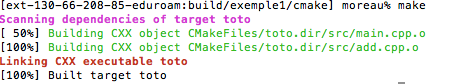
\includegraphics[width=8cm]{fig/cmake-snap1.png}
\end{center}

\end{frame}

\begin{frame}[fragile]\frametitle{Pour aller plus loin (1/2)}

\begin{itemize}
\itemsep1pt\parskip0pt\parsep0pt
\item
  générer l'exécutable dans le répertoire bin

  \begin{itemize}
  \itemsep1pt\parskip0pt\parsep0pt
  \item
    \texttt{set(EXECUTABLE\_OUTPUT\_PATH bin/\$\{CMAKE\_BUILD\_TYPE\})}
  \item
    permet en outre de spécifier une config Debug ou Release (pas vu
    ici)
  \end{itemize}
\item
  ne pas s'embêter à spécifier la liste des fichiers source
\begin{verbatim}
file( GLOB_RECURSE
  source_files
  src/*
)
add_executable ( toto $\{source_files\} )
\end{verbatim}
\item Si on ajoute un \texttt{.cpp}, il est nécessaire de relancer cmake pour regénérer le script de build, mais pas de toucher à la \texttt{CMakeLists.txt}
\end{itemize}

\end{frame}


\begin{frame}[fragile]\frametitle{Pour aller plus loin (2/2)}

\begin{itemize}
\itemsep1pt\parskip0pt\parsep0pt
\item
  générer des bibliothèques


  \begin{itemize}
  \itemsep1pt\parskip0pt\parsep0pt
  \item
    \texttt{add\_library( NOM TYPE fichiers sources)}
  \item
    où TYPE vaut SHARED ou STATIC
  \end{itemize}
\item sous-projets (pratique pour les librairies notamment)
\begin{itemize}
\item add\_subdirectory ( NOM )
\end{itemize}
\item Mais encore
\begin{itemize}
\item if(), endif() pour tester certaines conditions
\item macro() pour éviter de se répéter
\end{itemize}
\end{itemize}

\end{frame}

\begin{frame}{Utilisation d'IDE avec CMake}
\begin{itemize}
\item CMake sait générer des fichiers de projets pour des IDE modernes
\begin{itemize}
\item \texttt{cmake .. -G Xcode}
\end{itemize}
\end{itemize}
\begin{center}
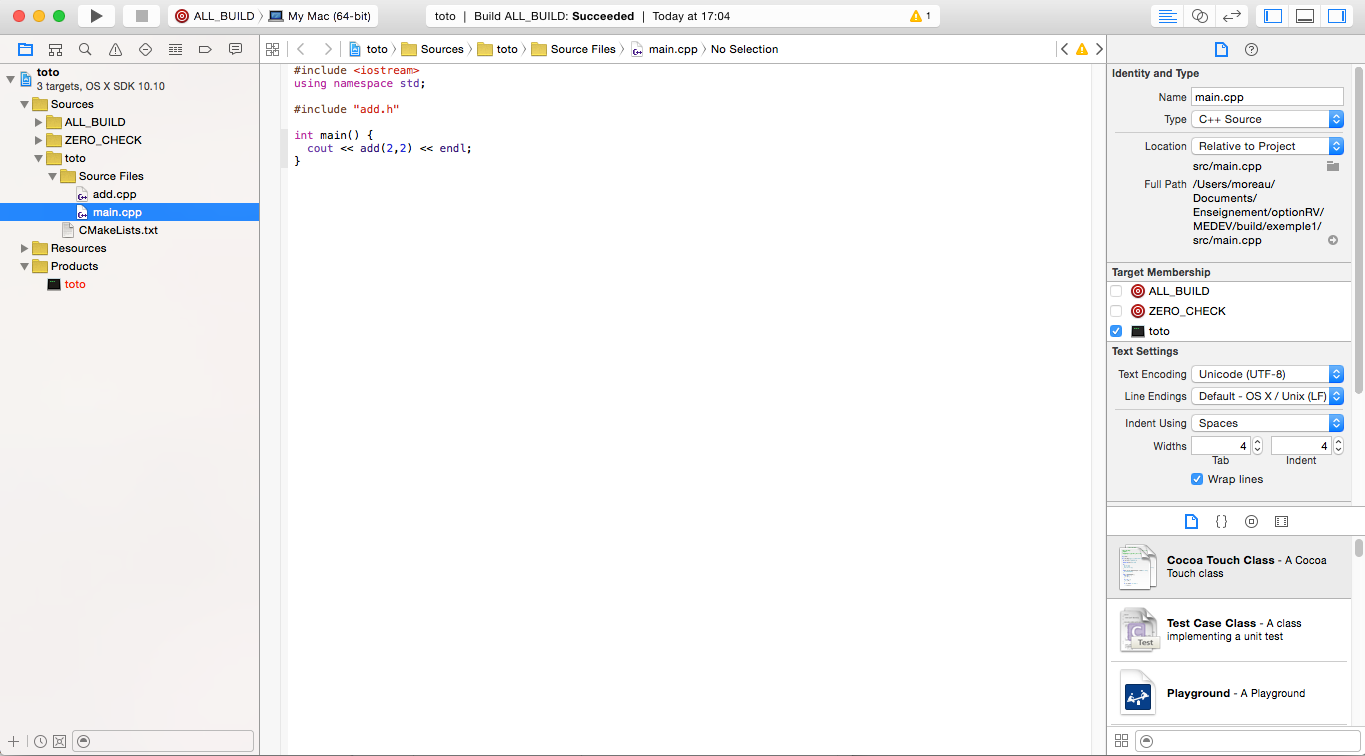
\includegraphics[width=8cm]{fig/cmake-xcode.png}
\end{center}
\end{frame}

\begin{frame}[fragile]\frametitle{Utilisation de bibliothèques externes}

\begin{itemize}
\itemsep1pt\parskip0pt\parsep0pt
\item
  Méthode manuelle

  \begin{itemize}
  \itemsep1pt\parskip0pt\parsep0pt
  \item
    compilation : utilisation de include\_directories ( \ldots{} )
  \item
    édition des liens : utilisation de

    \begin{itemize}
    \itemsep1pt\parskip0pt\parsep0pt
    \item
      link\_directories ( \ldots{} )
    \item
      target\_link\_directories ( toto \ldots{} )
    \end{itemize}
  \item
    NB : on pourrait faire ça pour OpenSceneGraph
  \item
    Mais il y a plus simple !
\begin{verbatim}
find_package ( OpenScenegraph VERSION REQUIRED composants )
INCLUDE_DIRECTORIES(${OPENSCENEGRAPH_INCLUDE_DIRS})
TARGET_LINK_LIBRARIES(toto ${OPENSCENEGRAPH_LIBRARIES})
\end{verbatim}
\item juste remplacer VERSION par une version minimum et composants par la liste des composants OSG obligatoires
\item La doc de CMake liste les variables définies par le package \href{http://www.cmake.org/cmake/help/v3.0/module/FindOpenSceneGraph.html}{OpenSceneGraph}
  \end{itemize}
\end{itemize}

\end{frame}

\begin{frame}{FindOpenSceneGraph}
\begin{center}
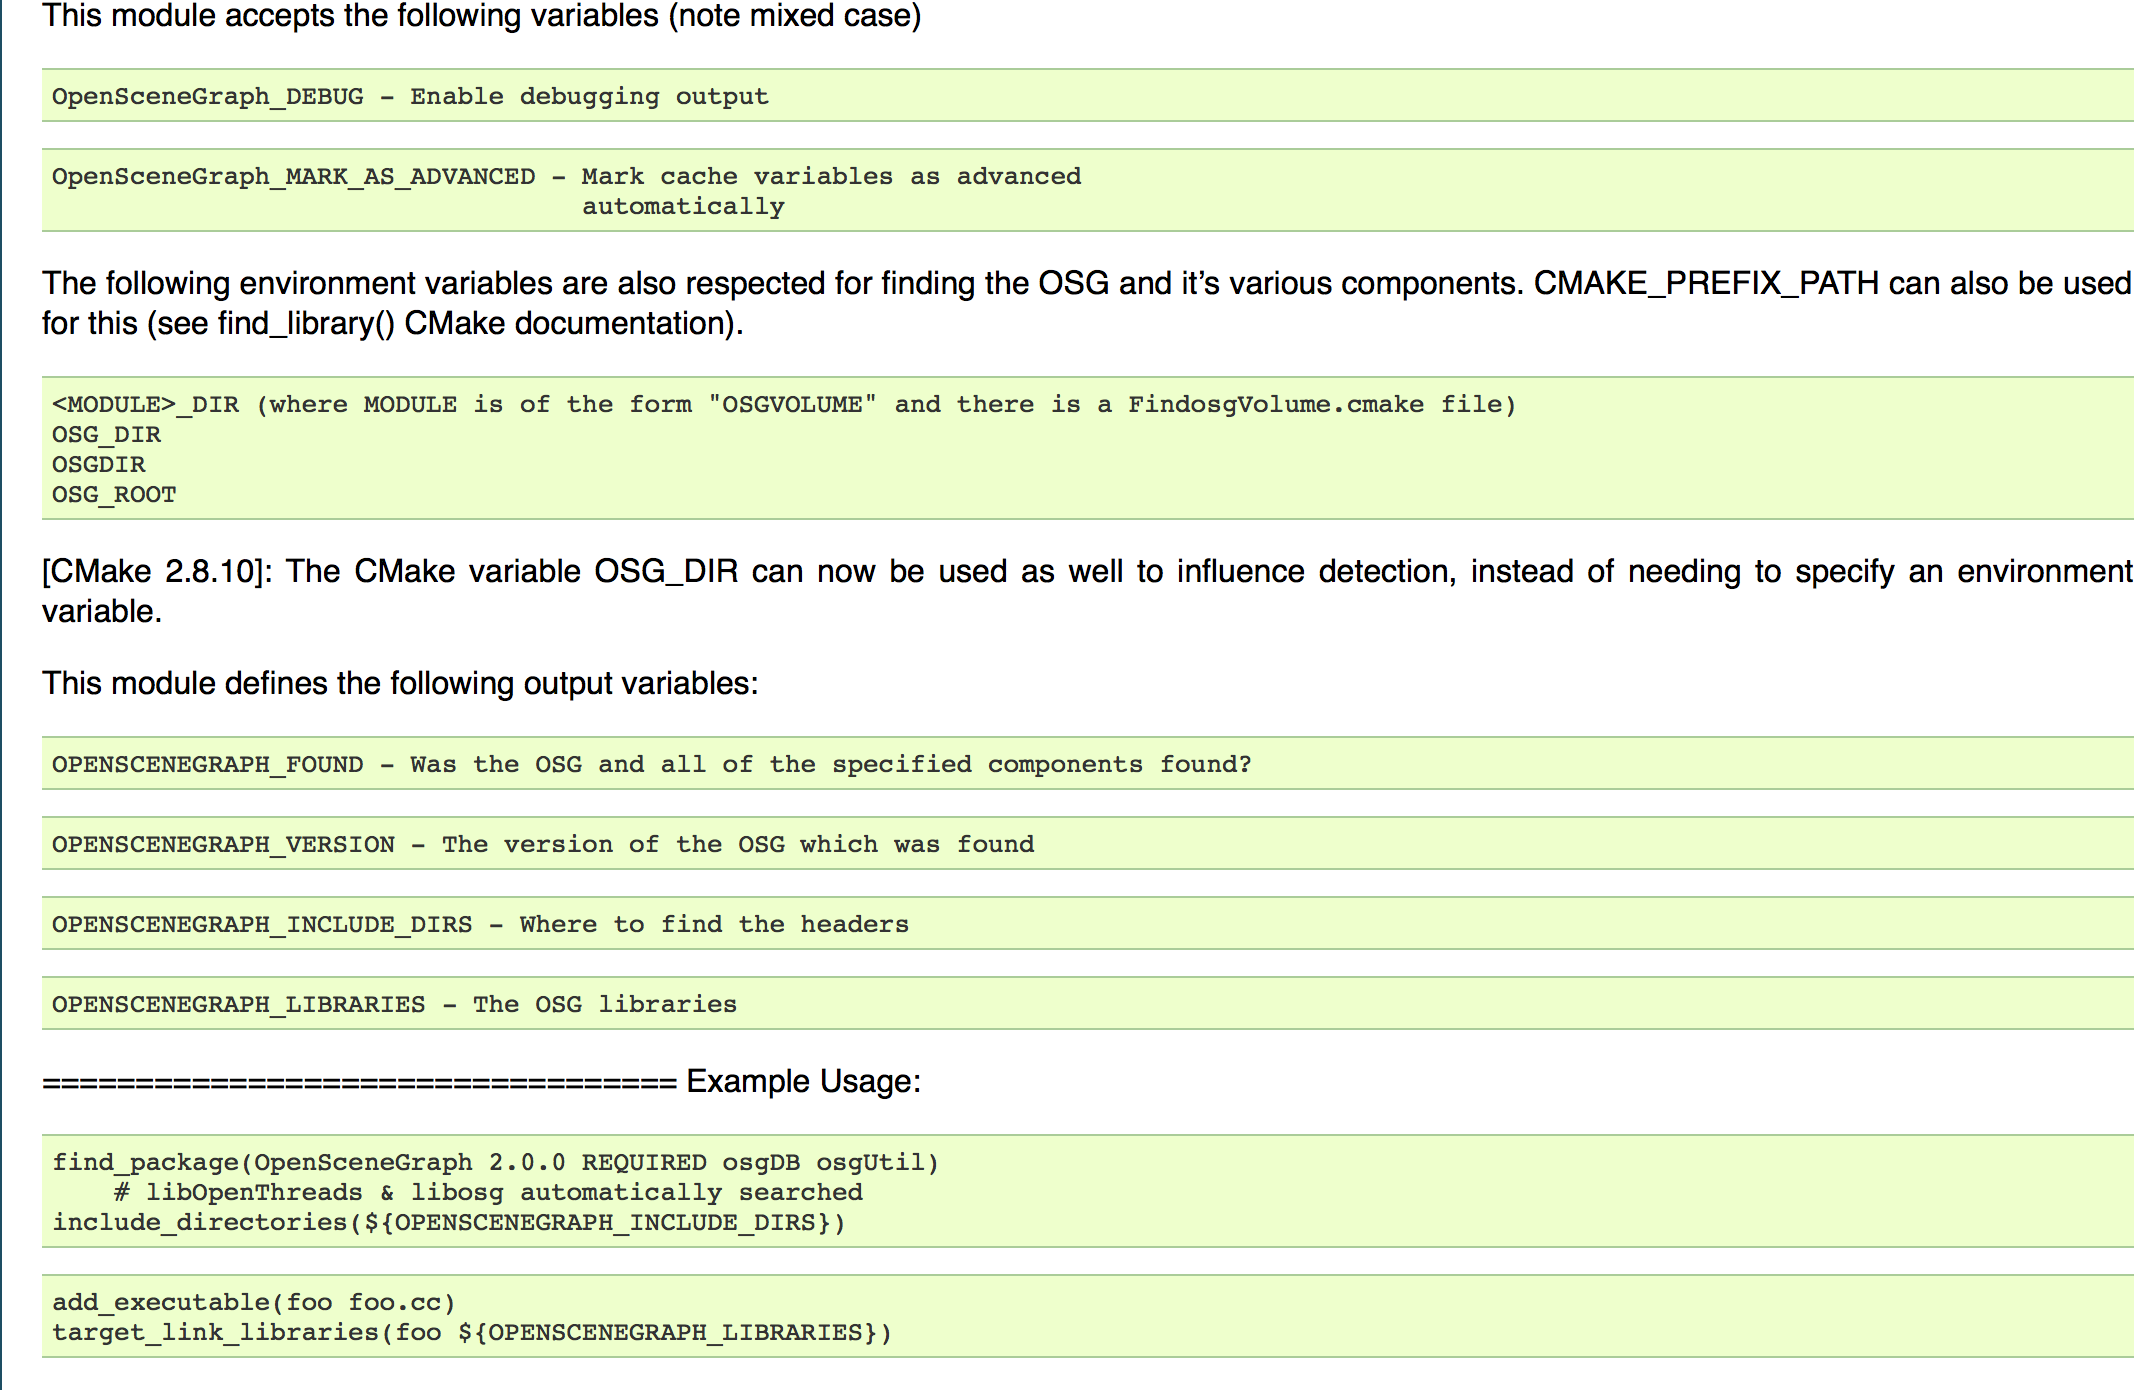
\includegraphics[width=9.5cm]{fig/FindOpenSceneGraph.png}

\end{center}\end{frame}

\begin{frame}{Quelques compléments sur CMake}

\begin{itemize}
\itemsep1pt\parskip0pt\parsep0pt
\item \href{http://www.cmake.org}{Site officiel}
\item \href{http://www.cmake.org/documentation/}{Documentation}
  \url{http://www.landofthebytes.com/?page\_id=358}
\item \url{http://florian-goujeon.developpez.com/cours/cmake/initiation/}
\end{itemize}

\end{frame}

\begin{frame}{TP du jour}
\begin{itemize}
\item On reprend un vieux  TP avions ...
\item Code rassemblé ici (avec un CMakeLists.txt) : \url{https://github.com/guillaumemoreau/TP-avions}
\item A faire
\begin{itemize}
\item Fork de ce repository
\item continuer / finir le TP dans son coin
\item Renvoyer l'adresse de son fork
\item indice : les tests unitaires ne sont pas interdits...
\end{itemize}
\end{itemize}
\end{frame}
